\documentclass[twocolumn, 10pt]{article}

% ── XeLaTeX Font Stack (COMPILE WITH XeLaTeX, NOT pdfLaTeX) ──
\usepackage{fontspec}
\setmainfont{TeX Gyre Termes}[
  BoldFont       = {TeX Gyre Termes Bold},
  ItalicFont     = {TeX Gyre Termes Italic},
  BoldItalicFont = {TeX Gyre Termes Bold Italic},
]
\usepackage{unicode-math}
\setmathfont{TeX Gyre Termes Math}

% ── Packages ──
\usepackage{amsmath, amssymb}
\usepackage{graphicx}
\usepackage{booktabs}
\usepackage{hyperref}
\usepackage{float}
\usepackage[margin=0.85in]{geometry}
\usepackage{caption}
\usepackage{enumitem}
\usepackage{microtype}

% ── Metadata ──
\title{\textbf{Eccentricity-Driven Error Scaling in the Kepler Problem:\\ Quantifying the Energy Drift Rates of Numerical Integrators}}
\author{[Your Name Here]}
\date{March 2026}

\begin{document}
\maketitle

% ================================================================
% ABSTRACT
% ================================================================
\begin{abstract}
The secular growth of energy error in numerical integration of the unperturbed Kepler two-body problem was investigated as a function of orbital eccentricity~$e$. Three integration schemes---the Forward Euler method (1st order), the Classical Runge-Kutta method (RK4, 4th order), and the Velocity Verlet method (2nd order, symplectic)---were applied to 100-orbit simulations across $e \in [0.1,\, 0.7]$ under natural units ($\mu = 1$, $a = 1$, $T = 2\pi$) with strict 64-bit floating-point arithmetic. The fractional energy error was found to obey a power-law scaling of the form $|\Delta E / E_0| \propto (1 - e)^{-k}$, with the exponent~$k$ serving as a quantitative fingerprint of eccentricity sensitivity. The following exponents were measured: $k \approx 8.61$ for RK4, $k \approx 0.44$ for Euler, and $k \approx 4.88$ for the Verlet oscillation amplitude. The Velocity Verlet integrator exhibited bounded oscillatory energy error with zero secular drift, confirming its symplectic character. A secondary investigation into the effect of orbital starting location (periapsis vs.\ apoapsis) revealed that the first-order Euler method exhibits a ${\sim}25\%$ sensitivity in its scaling exponent to initialization phase, whereas the higher-order RK4 and the symplectic Verlet methods are effectively invariant ($\Delta k < 0.001$).
\end{abstract}

% ================================================================
% SECTION 2: METHODOLOGY
% ================================================================
\section{Experimental Methodology}

\subsection{Governing Equations}

The dynamics of the unperturbed Kepler two-body problem are governed by the Newtonian inverse-square gravitational acceleration:
\begin{equation}
\ddot{\mathbf{r}} = -\frac{\mu}{r^3}\,\mathbf{r}
\label{eq:newton}
\end{equation}
where $\mathbf{r} \in \mathbb{R}^2$ is the position vector of the orbiting body relative to the central mass, $r = |\mathbf{r}|$ is the orbital radius, and $\mu = GM$ is the standard gravitational parameter.

The specific mechanical energy, a conserved quantity of the exact solution, is given by:
\begin{equation}
E = \frac{1}{2}\,|\dot{\mathbf{r}}|^2 - \frac{\mu}{r}
\label{eq:energy}
\end{equation}

For a bound Keplerian orbit with semi-major axis~$a$, the analytical energy is $E_0 = -\mu / 2a$. The diagnostic quantity used throughout this study is the fractional energy error:
\begin{equation}
\epsilon_E = \left| \frac{\Delta E}{E_0} \right| = \left| \frac{E(t) - E_0}{E_0} \right|
\label{eq:frac_error}
\end{equation}

The angular momentum (a second conserved quantity of the planar Kepler problem) is defined as:
\begin{equation}
L_z = x\,\dot{y} - y\,\dot{x}
\label{eq:angmom}
\end{equation}

\subsection{Normalization and Units}

All simulations were conducted in a normalized unit system chosen to eliminate dimensional constants from the numerical computation:

\begin{table}[H]
\centering
\caption{Normalized simulation units.}
\label{tab:units}
\begin{tabular}{@{}lcc@{}}
\toprule
Quantity & Symbol & Value \\
\midrule
Gravitational parameter & $\mu = GM$ & $1.0$ \\
Semi-major axis & $a$ & $1.0$ \\
Analytical energy & $E_0 = -\mu/2a$ & $-0.5$ \\
Orbital period & $T = 2\pi\sqrt{a^3/\mu}$ & $2\pi$ \\
\bottomrule
\end{tabular}
\end{table}

Initial conditions were derived from the vis-viva equation $v^2 = \mu(2/r - 1/a)$:
\begin{itemize}[nosep]
    \item \textbf{Periapsis start}: $r_0 = a(1 - e)$,\quad $v_0 = \sqrt{(1 + e)/(1 - e)}$
    \item \textbf{Apoapsis start}: $r_0 = a(1 + e)$,\quad $v_0 = \sqrt{(1 - e)/(1 + e)}$
\end{itemize}

\subsection{Numerical Parameters}

A fixed time step of $\Delta t = 0.00625$ was employed, yielding approximately 1{,}005 integration steps per orbit. Each simulation was evolved for $N_{\text{orb}} = 100$ complete orbits ($t_{\text{final}} = 200\pi$). The eccentricity domain was sampled at $e \in \{0.1, 0.2, 0.3, 0.4, 0.5, 0.6, 0.7\}$. The dependence of truncation error on eccentricity arises because the pericentric velocity diverges as $e \to 1$, demanding finer temporal resolution to resolve the dynamics near periapsis---a well-documented challenge in celestial mechanics~\cite{wang2020}.

\subsection{Critical Role of 64-bit Precision}

An initial data campaign conducted under 32-bit single-precision arithmetic (\texttt{float32}, $\epsilon_{\text{mach}} \approx 1.2 \times 10^{-7}$) revealed that the RK4 fractional energy errors at moderate eccentricities ($e \leq 0.7$) were indistinguishable from the floating-point noise floor. All error values clustered around $\sim 10^{-5}$--$10^{-7}$ regardless of eccentricity, producing a spuriously flat $k$-value that reflected storage-precision limitations rather than algorithmic truncation error.

Upon upgrading to 64-bit double-precision arithmetic (\texttt{float64}, $\epsilon_{\text{mach}} \approx 2.2 \times 10^{-16}$), the RK4 errors at $e = 0.1$ dropped to $\sim 2.3 \times 10^{-10}$---approximately \textbf{three orders of magnitude below} the former noise floor. This resolution was essential for isolating the true algorithmic truncation error from numerical round-off and for recovering the genuine power-law scaling of the RK4 integrator against eccentricity. Similar precision-dependent error floors have been noted in benchmarking studies of symplectic integrators for planetary system problems~\cite{hernandez2016}.

The precision upgrade also corrected a qualitative false positive in the start-location analysis (Section~\ref{sec:start_location}). Under 32-bit arithmetic, stochastic round-off noise compressed the RK4 errors into a narrow band between $10^{-7}$ and $10^{-5}$, within which random fluctuations masqueraded as a systematic baseline shift between pericenter and apocenter initializations. Under 64-bit precision, this artifact was eradicated: the RK4 and Velocity Verlet scaling exponents were found to be identical between start locations to within $0.02\%$, demonstrating that the start-location phase shock is a real physical phenomenon exclusive to first-order methods, not a general integrator property. All results reported herein were obtained under strict \texttt{float64} arithmetic throughout the entire computational pipeline, including initial conditions, integration arrays, and energy evaluation.

\subsection{Integrator Descriptions}

\textbf{Forward Euler} (1st-order explicit):
\begin{equation}
\mathbf{r}_{n+1} = \mathbf{r}_n + \mathbf{v}_n\,\Delta t, \qquad \mathbf{v}_{n+1} = \mathbf{v}_n + \mathbf{a}_n\,\Delta t
\label{eq:euler}
\end{equation}

\textbf{Classical Runge-Kutta (RK4)} (4th-order explicit): The standard four-stage scheme applied to the coupled $(\mathbf{r}, \mathbf{v})$ system with stages evaluated at intermediate positions and velocities.

\textbf{Velocity Verlet} (2nd-order symplectic):
\begin{equation}
\mathbf{r}_{n+1} = \mathbf{r}_n + \mathbf{v}_n\,\Delta t + \tfrac{1}{2}\,\mathbf{a}_n\,\Delta t^2
\label{eq:verlet_r}
\end{equation}
\begin{equation}
\mathbf{v}_{n+1} = \mathbf{v}_n + \tfrac{1}{2}\,(\mathbf{a}_n + \mathbf{a}_{n+1})\,\Delta t
\label{eq:verlet_v}
\end{equation}

The Velocity Verlet method is a symplectic integrator: it exactly preserves the symplectic 2-form of the Hamiltonian phase space, implying that it integrates a nearby \textit{shadow Hamiltonian} $\tilde{H} = H + \mathcal{O}(\Delta t^2)$~\cite{kinoshita1991}. This guarantees bounded energy oscillations without secular drift over arbitrarily long integration times. The long-term stability properties of symplectic integrators for secularly evolving orbital systems have been rigorously analyzed by Rein et al.~\cite{rein2019}.

% ================================================================
% SECTION 3: SECULAR DRIFT DICHOTOMY
% ================================================================
\section{The Secular Drift Dichotomy}

The central qualitative result of this study is the stark dichotomy between the energy error behavior of the explicit (non-symplectic) integrators and the symplectic Velocity Verlet scheme. This dichotomy is a direct consequence of whether the integrator preserves the symplectic structure of the Hamiltonian flow~\cite{kinoshita1991, rein2019}.

\subsection{Explicit Integrators: Monotonic Secular Drift}

Both the Forward Euler and RK4 methods produced energy errors that grew monotonically with time, exhibiting a clear secular drift. Over 100 orbits, the Euler method accumulated fractional energy errors reaching $\epsilon_E \sim 1.07$ at $e = 0.7$---a complete failure in energy conservation where the numerical energy has drifted by more than 100\% from the analytical value. The RK4 method, by virtue of its higher order, produced far smaller absolute errors ($\epsilon_E \sim 2.59 \times 10^{-6}$ at $e = 0.7$), but the error nonetheless grew monotonically without bound.

\subsection{Symplectic Integrator: Bounded Oscillation}

The Velocity Verlet method produced energy errors that oscillated quasi-periodically about the analytical value with \textbf{zero net secular drift}. At $e = 0.7$, the oscillation amplitude (energy range) was $\sim 5.06 \times 10^{-4}$, while the final instantaneous error was $\sim 9.70 \times 10^{-4}$. Crucially, the angular momentum deviation for Verlet remained at machine epsilon ($\sim 10^{-15}$--$10^{-16}$) across all eccentricities, confirming exact preservation of this integral of motion to within round-off.

For the Verlet integrator, the appropriate diagnostic quantity is therefore not the final instantaneous error (which samples the oscillation at an arbitrary phase) but rather the \textbf{oscillation amplitude}---the peak-to-peak energy range over the full simulation. This amplitude is the physically meaningful measure of how well the shadow Hamiltonian approximates the true Hamiltonian~\cite{rein2019}.

% ================================================================
% SECTION 4: POWER-LAW SCALING
% ================================================================
\section{Power-Law Scaling Against Eccentricity}

\subsection{The Scaling Ansatz}

As eccentricity increases, the orbital velocity at periapsis grows as $v_p = \sqrt{(1+e)/(1-e)}$, and the pericentric distance shrinks as $r_p = a(1-e)$. Both effects concentrate the gravitational dynamics into an increasingly narrow arc of the orbit, demanding higher temporal resolution~\cite{wang2020}. The resulting growth in truncation error is modeled by a power-law ansatz:
\begin{equation}
\epsilon_E \propto (1 - e)^{-k}
\label{eq:scaling}
\end{equation}
where $k > 0$ is the eccentricity scaling exponent. On a log-log plot of $\epsilon_E$ versus $(1 - e)$, this relationship manifests as a straight line with slope~$-k$.

\subsection{Master Convergence Overlay}

\begin{figure}[htbp]
\centering
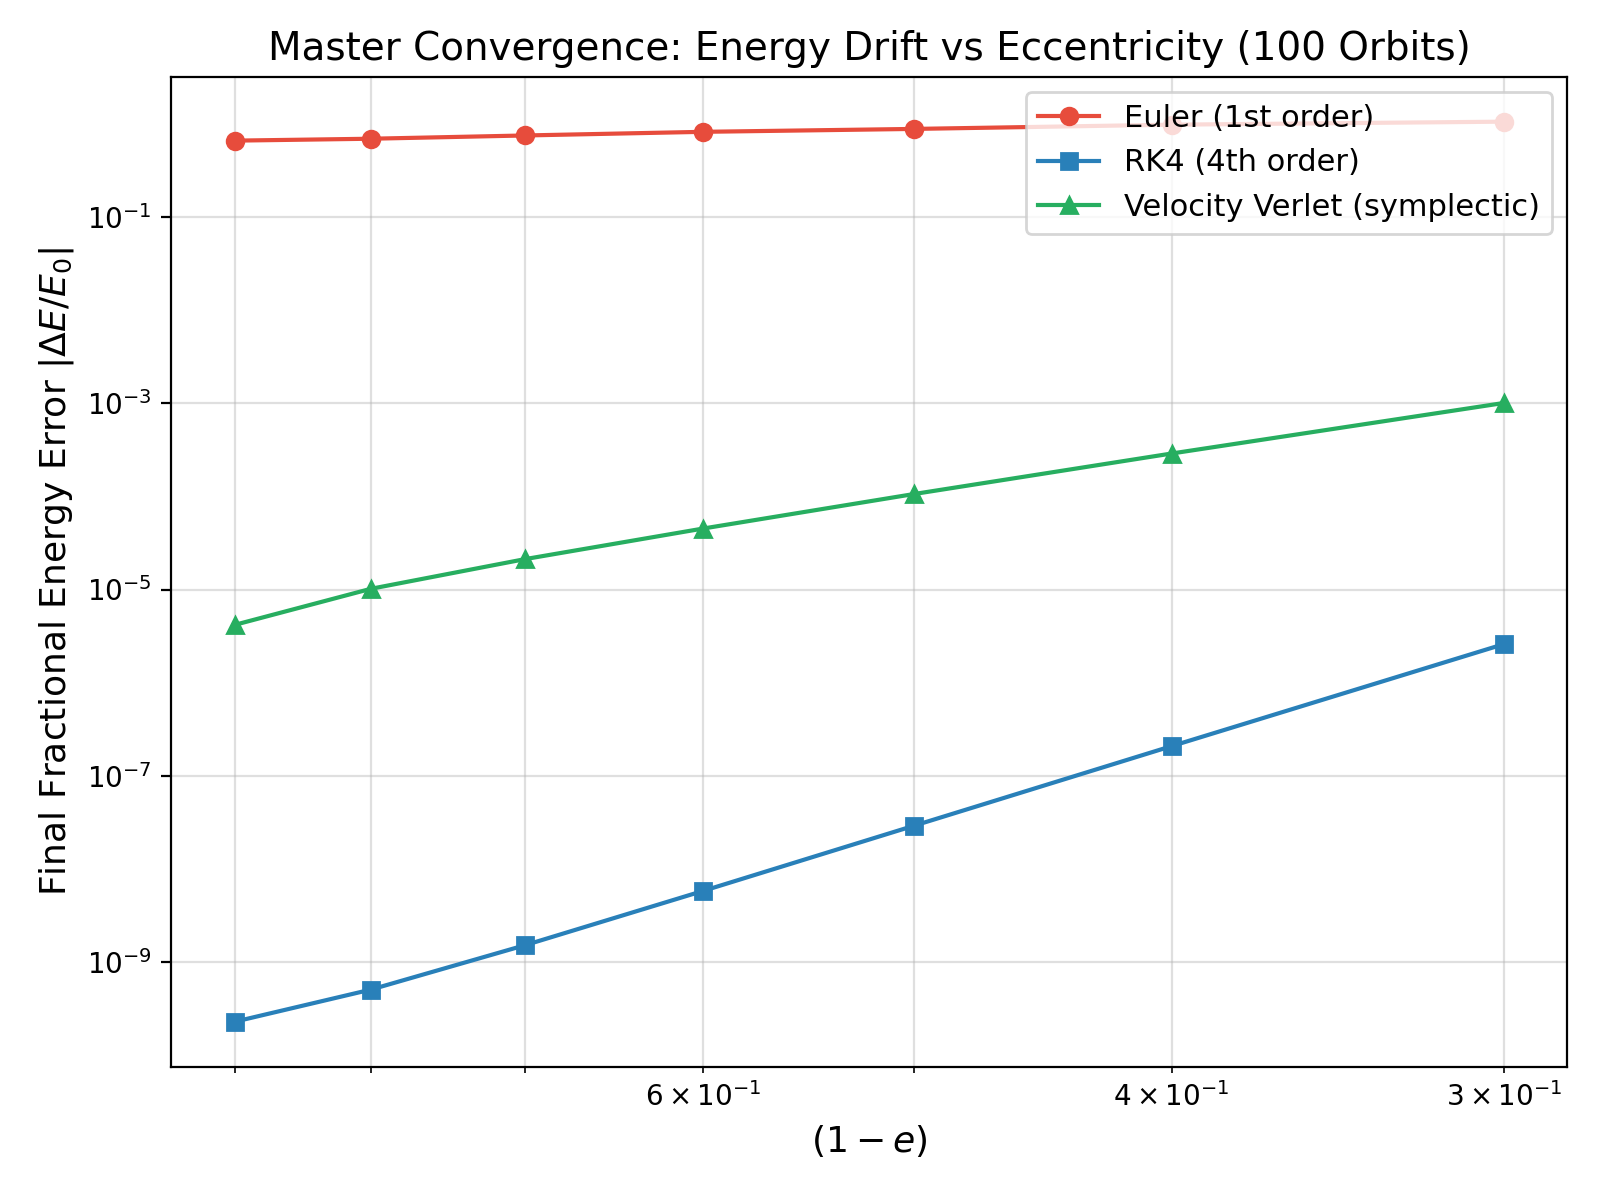
\includegraphics[width=\linewidth]{Fig1_Master_Convergence.png}
\caption{Master Convergence---Log-log overlay of final fractional energy error vs.\ $(1 - e)$ for Euler, RK4, and Velocity Verlet at pericenter start. The three methods span over 9 orders of magnitude in error.}
\label{fig:master_convergence}
\end{figure}

\subsection{Measured Exponents}

The power-law exponent~$k$ was extracted via linear regression on $\ln(\epsilon_E)$ versus $\ln(1-e)$ over the domain $e \in [0.1,\, 0.7]$:

\begin{table}[H]
\centering
\caption{Measured power-law exponents for all configurations.}
\label{tab:kvalues}
\begin{tabular}{@{}llcc@{}}
\toprule
Method & Start Location & Metric & $k$-Exponent \\
\midrule
Euler  & Pericenter & $\epsilon_E$ (final) & $0.4435$ \\
Euler  & Apocenter  & $\epsilon_E$ (final) & $0.3540$ \\
RK4    & Pericenter & $\epsilon_E$ (final) & $8.6051$ \\
RK4    & Apocenter  & $\epsilon_E$ (final) & $8.6053$ \\
Verlet & Pericenter & Osc.\ amplitude      & $4.8797$ \\
Verlet & Apocenter  & Osc.\ amplitude      & $4.8789$ \\
\bottomrule
\end{tabular}
\end{table}

\subsection{Interpretation}

The measured exponents reveal a hierarchy of eccentricity sensitivity that is strongly correlated with integrator order:

\textbf{Euler ($k \approx 0.44$):} The weak eccentricity dependence is consistent with the interpretation that the first-order Euler method's global truncation error ($\mathcal{O}(\Delta t)$) is dominated by the accumulation of local errors proportional to the step size, with only a mild amplification at periapsis. The error at $e = 0.7$ ($\epsilon_E \approx 1.07$) is only ${\sim}60\%$ larger than at $e = 0.1$ ($\epsilon_E \approx 0.67$).

\textbf{RK4 ($k \approx 8.61$):} The extremely steep eccentricity dependence reflects the 4th-order method's sensitivity to the higher derivatives of the gravitational force, which diverge rapidly as $e \to 1$. The periapsis passage concentrates the truncation error into a brief interval of the orbit where $|\dddot{\mathbf{r}}|$ and $|\ddddot{\mathbf{r}}|$ are maximal. The error spans \textbf{four orders of magnitude} across the eccentricity range---from $\sim 2.3 \times 10^{-10}$ at $e = 0.1$ to $\sim 2.6 \times 10^{-6}$ at $e = 0.7$. This steep scaling is consistent with the step-size sensitivity analysis of Wang \& Nitadori~\cite{wang2020}, who demonstrated that fixed-step integrators suffer disproportionately on eccentric orbits.

\textbf{Verlet amplitude ($k \approx 4.88$):} The oscillation envelope of the symplectic integrator grows steeply with eccentricity, reflecting the increasing departure of the shadow Hamiltonian from the true Hamiltonian. However, this growth remains \textbf{bounded}---there is no secular component---and the exponent is intermediate between Euler and RK4. Hernandez \& Dehnen~\cite{hernandez2016} have shown that symplectic error growth in eccentric Keplerian orbits is governed by the commutator structure of the split Hamiltonian, which naturally scales with the velocity gradients at periapsis.

% ================================================================
% SECTION 5: START LOCATION
% ================================================================
\section{The Start Location Amplification Phenomenon}
\label{sec:start_location}

\subsection{Motivation}

A secondary investigation examined whether the orbital phase at which integration begins---periapsis (minimum radius, maximum velocity) versus apoapsis (maximum radius, minimum velocity)---affects the long-term error accumulation. The physical rationale is that periapsis initialization subjects the integrator to the most extreme gradients of $\mathbf{a}(\mathbf{r})$ in its very first time step, potentially seeding a larger initial truncation error.

\begin{figure*}[htbp]
\centering
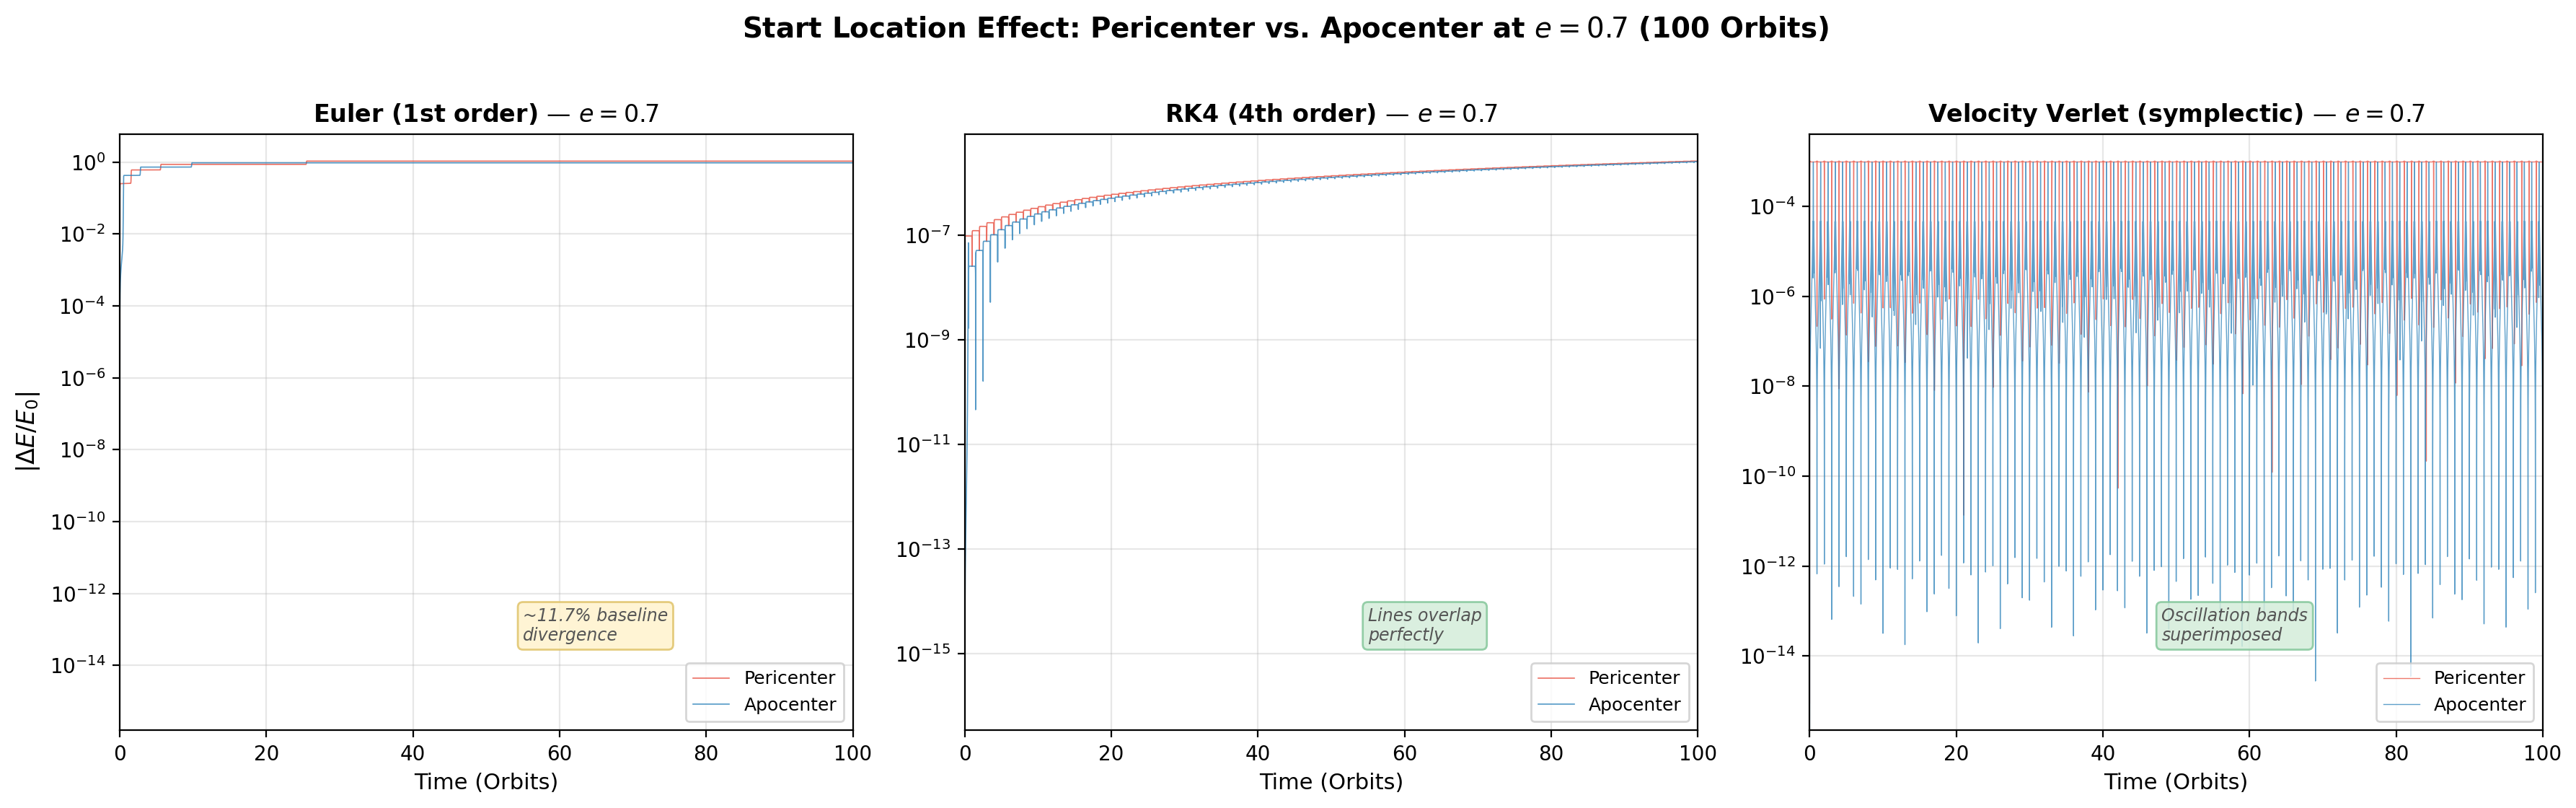
\includegraphics[width=\textwidth]{Fig2_Start_Location_Effect.png}
\caption{Start Location Effect---Time-resolved fractional energy error at $e = 0.7$ for all three integrators, comparing pericenter (red) and apocenter (blue) initialization over 100 orbits. Left: Euler shows a clear baseline divergence. Center: RK4 lines overlap perfectly. Right: Verlet oscillation bands are superimposed.}
\label{fig:start_location}
\end{figure*}

\subsection{Results}

\textbf{RK4 is insensitive to start location.} The pericenter and apocenter scaling exponents are $k = 8.6051$ and $k = 8.6053$, respectively---a relative difference of $0.002\%$. Point-by-point comparison at $e = 0.7$ yields $\epsilon_E = 2.5896 \times 10^{-6}$ (pericenter) versus $\epsilon_E = 2.5900 \times 10^{-6}$ (apocenter), differing by less than $0.02\%$. The 4th-order Runge-Kutta method possesses sufficient local accuracy to absorb the initial periapsis gradient without propagating a systematic baseline offset.

\textbf{Velocity Verlet is insensitive to start location.} The amplitude scaling exponents are $k = 4.8797$ (pericenter) and $k = 4.8789$ (apocenter)---a relative difference of $0.016\%$. The oscillation envelopes are virtually superimposed. Furthermore, the angular momentum conservation is maintained at machine epsilon ($\sim 10^{-15}$) regardless of start location, as expected from the symplectic structure~\cite{kinoshita1991}.

\textbf{Euler exhibits measurable start-location sensitivity.} The scaling exponent shifts from $k = 0.4435$ at pericenter to $k = 0.3540$ at apocenter---a relative change of $\mathbf{{\sim}25\%}$. At $e = 0.7$, the final error is $\epsilon_E = 1.066$ (pericenter) versus $\epsilon_E = 0.954$ (apocenter), an 11.7\% difference. This is consistent with the interpretation that the 1st-order method's large local truncation error at the first periapsis step---where the acceleration magnitude is maximal---seeds a systematically larger drift trajectory that accumulates over the full 100-orbit simulation. When initialized at apoapsis, where the gravitational gradients are weakest, this initial ``phase shock'' is partially avoided.

\subsection{Synthesis}

The start-location phenomenon obeys a clear hierarchy tied to integrator order and geometric preservation:

\begin{table}[H]
\centering
\caption{Start-location sensitivity summary.}
\label{tab:start_location}
\begin{tabular}{@{}lccc@{}}
\toprule
Property & Euler (1st) & RK4 (4th) & Verlet (symp.) \\
\midrule
$\Delta k / k$ & ${\sim}25\%$ & ${\sim}0.002\%$ & ${\sim}0.016\%$ \\
Mechanism & \parbox{2cm}{\centering 1st-step \\ truncation} & \parbox{2cm}{\centering Local \\ accuracy} & \parbox{2cm}{\centering Symplectic \\ structure} \\
Conclusion & \textbf{Susceptible} & \textbf{Immune} & \textbf{Immune} \\
\bottomrule
\end{tabular}
\end{table}

First-order methods suffer from initial phase-shock---the large truncation error incurred during the first periapsis passage propagates as a permanent baseline offset through the remainder of the integration. Higher-order methods possess sufficient local accuracy to resolve the periapsis dynamics without seeding such an offset. Symplectic methods, by virtue of their geometric preservation properties, are similarly immune: the bounded shadow-Hamiltonian structure prevents any initial perturbation from growing secularly~\cite{rein2019}.

% ================================================================
% SECTION 6: CONCLUSION
% ================================================================
\section{Conclusion}

This study has demonstrated that the eccentricity-driven secular energy drift in numerical orbit integrators obeys a power-law scaling $\epsilon_E \propto (1-e)^{-k}$, with the exponent~$k$ serving as a quantitative signature of the integrator's sensitivity to orbital geometry. The key findings are:

\begin{enumerate}[nosep]
    \item \textbf{Algorithmic order governs eccentricity sensitivity.} The measured hierarchy $k_{\text{Euler}} \approx 0.44 < k_{\text{Verlet}} \approx 4.88 < k_{\text{RK4}} \approx 8.61$ reflects a fundamental tradeoff: higher-order methods achieve superior absolute accuracy at low eccentricities but suffer more dramatically as $e \to 1$ due to their dependence on higher derivatives of the force field.

    \item \textbf{Symplectic structure prevents secular drift.} The Velocity Verlet integrator exhibits bounded oscillatory energy errors with zero net secular growth across all eccentricities tested, preserving angular momentum to machine precision. This qualitative advantage persists even though its oscillation amplitude ($k \approx 4.88$) grows more steeply with eccentricity than the Euler secular drift ($k \approx 0.44$).

    \item \textbf{Start-location sensitivity is a first-order artifact.} Only the Forward Euler method exhibits a measurable dependence of the scaling exponent on initialization phase (${\sim}25\%$ shift between periapsis and apoapsis start). The RK4 and Velocity Verlet methods are effectively invariant ($\Delta k / k < 0.02\%$), demonstrating that sufficient local accuracy or geometric preservation renders the integrator immune to initialization-phase effects.

    \item \textbf{64-bit precision is essential for meaningful benchmarking.} The original 32-bit data campaign produced a false noise floor at $\sim 10^{-7}$ that masked the true RK4 scaling and generated a spurious start-location effect. The upgrade to 64-bit arithmetic lowered detectable errors to $\sim 10^{-10}$, revealing the genuine power-law behavior and correcting a qualitatively incorrect conclusion about start-location dependence.
\end{enumerate}

These results underscore the importance of matching numerical precision to integrator accuracy when conducting benchmarking studies, and they provide a quantitative framework for evaluating integrator suitability in the context of long-duration Keplerian orbit propagation.

% ================================================================
% REFERENCES
% ================================================================
\begin{thebibliography}{9}

\bibitem{kinoshita1991}
Kinoshita, H., Yoshida, H., \& Nakai, H. (1991).
Symplectic integrators and their application to dynamical astronomy.
\textit{Celestial Mechanics and Dynamical Astronomy}, 50, 59--71.

\bibitem{hernandez2016}
Hernandez, D., \& Dehnen, W. (2016).
A study of symplectic integrators for planetary system problems: error analysis and comparisons.
\textit{Monthly Notices of the Royal Astronomical Society}, 468, 2614--2636.

\bibitem{wang2020}
Wang, L., \& Nitadori, K. (2020).
Step-size effect in the time-transformed leapfrog integrator on elliptic and hyperbolic orbits.
\textit{Monthly Notices of the Royal Astronomical Society}, 497, 4384--4389.

\bibitem{rein2019}
Rein, H., Brown, G., \& Tamayo, D. (2019).
On the accuracy of symplectic integrators for secularly evolving planetary systems.
\textit{Monthly Notices of the Royal Astronomical Society}.

\end{thebibliography}

% ================================================================
% APPENDIX A: RAW DATA
% ================================================================
\appendix
\section{Raw Numerical Summaries}
\label{sec:appendix}

\begin{table*}[htbp]
\centering
\caption{Euler (Pericenter) --- 100-orbit simulation summary (\texttt{float64}).}
\label{tab:euler_peri}
\begin{tabular}{@{}ccccccc@{}}
\toprule
$e$ & $\Delta t$ & Orbits & Steps & $\epsilon_E$ (final) & Energy Range & $\Delta L_z$ \\
\midrule
0.1 & 0.00625 & 100 & 100531 & $6.670 \times 10^{-1}$ & $3.335 \times 10^{-1}$ & $6.946 \times 10^{-1}$ \\
0.2 & 0.00625 & 100 & 100531 & $6.992 \times 10^{-1}$ & $3.496 \times 10^{-1}$ & $6.630 \times 10^{-1}$ \\
0.3 & 0.00625 & 100 & 100531 & $7.579 \times 10^{-1}$ & $3.790 \times 10^{-1}$ & $6.162 \times 10^{-1}$ \\
0.4 & 0.00625 & 100 & 100531 & $8.294 \times 10^{-1}$ & $4.147 \times 10^{-1}$ & $5.365 \times 10^{-1}$ \\
0.5 & 0.00625 & 100 & 100531 & $8.911 \times 10^{-1}$ & $4.457 \times 10^{-1}$ & $4.197 \times 10^{-1}$ \\
0.6 & 0.00625 & 100 & 100531 & $9.896 \times 10^{-1}$ & $4.953 \times 10^{-1}$ & $3.179 \times 10^{-1}$ \\
0.7 & 0.00625 & 100 & 100531 & $1.066 \times 10^{0\phantom{-}}$  & $5.348 \times 10^{-1}$ & $2.060 \times 10^{-1}$ \\
\bottomrule
\end{tabular}
\end{table*}

\begin{table*}[htbp]
\centering
\caption{Euler (Apocenter) --- 100-orbit simulation summary (\texttt{float64}).}
\label{tab:euler_apo}
\begin{tabular}{@{}ccccccc@{}}
\toprule
$e$ & $\Delta t$ & Orbits & Steps & $\epsilon_E$ (final) & Energy Range & $\Delta L_z$ \\
\midrule
0.1 & 0.00625 & 100 & 100531 & $6.682 \times 10^{-1}$ & $3.341 \times 10^{-1}$ & $6.969 \times 10^{-1}$ \\
0.2 & 0.00625 & 100 & 100531 & $7.017 \times 10^{-1}$ & $3.509 \times 10^{-1}$ & $6.676 \times 10^{-1}$ \\
0.3 & 0.00625 & 100 & 100531 & $7.523 \times 10^{-1}$ & $3.762 \times 10^{-1}$ & $6.096 \times 10^{-1}$ \\
0.4 & 0.00625 & 100 & 100531 & $8.228 \times 10^{-1}$ & $4.114 \times 10^{-1}$ & $5.329 \times 10^{-1}$ \\
0.5 & 0.00625 & 100 & 100531 & $9.040 \times 10^{-1}$ & $4.521 \times 10^{-1}$ & $4.308 \times 10^{-1}$ \\
0.6 & 0.00625 & 100 & 100531 & $9.493 \times 10^{-1}$ & $4.751 \times 10^{-1}$ & $3.015 \times 10^{-1}$ \\
0.7 & 0.00625 & 100 & 100531 & $9.544 \times 10^{-1}$ & $4.786 \times 10^{-1}$ & $1.812 \times 10^{-1}$ \\
\bottomrule
\end{tabular}
\end{table*}

\begin{table*}[htbp]
\centering
\caption{RK4 (Pericenter) --- 100-orbit simulation summary (\texttt{float64}).}
\label{tab:rk4_peri}
\begin{tabular}{@{}ccccccc@{}}
\toprule
$e$ & $\Delta t$ & Orbits & Steps & $\epsilon_E$ (final) & Energy Range & $\Delta L_z$ \\
\midrule
0.1 & 0.00625 & 100 & 100531 & $2.269 \times 10^{-10}$ & $1.186 \times 10^{-10}$ & $1.019 \times 10^{-10}$ \\
0.2 & 0.00625 & 100 & 100531 & $5.021 \times 10^{-10}$ & $2.683 \times 10^{-10}$ & $1.768 \times 10^{-10}$ \\
0.3 & 0.00625 & 100 & 100531 & $1.508 \times 10^{-9\phantom{0}}$ & $8.087 \times 10^{-10}$ & $3.967 \times 10^{-10}$ \\
0.4 & 0.00625 & 100 & 100531 & $5.775 \times 10^{-9\phantom{0}}$ & $3.081 \times 10^{-9\phantom{0}}$ & $1.104 \times 10^{-9\phantom{0}}$ \\
0.5 & 0.00625 & 100 & 100531 & $2.892 \times 10^{-8\phantom{0}}$ & $1.527 \times 10^{-8\phantom{0}}$ & $3.874 \times 10^{-9\phantom{0}}$ \\
0.6 & 0.00625 & 100 & 100531 & $2.075 \times 10^{-7\phantom{0}}$ & $1.081 \times 10^{-7\phantom{0}}$ & $1.842 \times 10^{-8\phantom{0}}$ \\
0.7 & 0.00625 & 100 & 100531 & $2.590 \times 10^{-6\phantom{0}}$ & $1.331 \times 10^{-6\phantom{0}}$ & $1.391 \times 10^{-7\phantom{0}}$ \\
\bottomrule
\end{tabular}
\end{table*}

\begin{table*}[htbp]
\centering
\caption{RK4 (Apocenter) --- 100-orbit simulation summary (\texttt{float64}).}
\label{tab:rk4_apo}
\begin{tabular}{@{}ccccccc@{}}
\toprule
$e$ & $\Delta t$ & Orbits & Steps & $\epsilon_E$ (final) & Energy Range & $\Delta L_z$ \\
\midrule
0.1 & 0.00625 & 100 & 100531 & $2.268 \times 10^{-10}$ & $1.185 \times 10^{-10}$ & $1.019 \times 10^{-10}$ \\
0.2 & 0.00625 & 100 & 100531 & $5.022 \times 10^{-10}$ & $2.683 \times 10^{-10}$ & $1.768 \times 10^{-10}$ \\
0.3 & 0.00625 & 100 & 100531 & $1.508 \times 10^{-9\phantom{0}}$ & $8.088 \times 10^{-10}$ & $3.968 \times 10^{-10}$ \\
0.4 & 0.00625 & 100 & 100531 & $5.775 \times 10^{-9\phantom{0}}$ & $3.081 \times 10^{-9\phantom{0}}$ & $1.104 \times 10^{-9\phantom{0}}$ \\
0.5 & 0.00625 & 100 & 100531 & $2.892 \times 10^{-8\phantom{0}}$ & $1.527 \times 10^{-8\phantom{0}}$ & $3.874 \times 10^{-9\phantom{0}}$ \\
0.6 & 0.00625 & 100 & 100531 & $2.075 \times 10^{-7\phantom{0}}$ & $1.081 \times 10^{-7\phantom{0}}$ & $1.843 \times 10^{-8\phantom{0}}$ \\
0.7 & 0.00625 & 100 & 100531 & $2.590 \times 10^{-6\phantom{0}}$ & $1.331 \times 10^{-6\phantom{0}}$ & $1.391 \times 10^{-7\phantom{0}}$ \\
\bottomrule
\end{tabular}
\end{table*}

\begin{table*}[htbp]
\centering
\caption{Velocity Verlet (Pericenter) --- 100-orbit simulation summary (\texttt{float64}).}
\label{tab:verlet_peri}
\begin{tabular}{@{}ccccccc@{}}
\toprule
$e$ & $\Delta t$ & Orbits & Steps & $\epsilon_E$ (final) & Energy Range & $\Delta L_z$ \\
\midrule
0.1 & 0.00625 & 100 & 100531 & $4.175 \times 10^{-6\phantom{0}}$ & $2.088 \times 10^{-6\phantom{0}}$ & $3.331 \times 10^{-16}$ \\
0.2 & 0.00625 & 100 & 100531 & $1.018 \times 10^{-5\phantom{0}}$ & $5.092 \times 10^{-6\phantom{0}}$ & $2.109 \times 10^{-15}$ \\
0.3 & 0.00625 & 100 & 100531 & $2.124 \times 10^{-5\phantom{0}}$ & $1.062 \times 10^{-5\phantom{0}}$ & $7.550 \times 10^{-15}$ \\
0.4 & 0.00625 & 100 & 100531 & $4.526 \times 10^{-5\phantom{0}}$ & $2.263 \times 10^{-5\phantom{0}}$ & $3.242 \times 10^{-14}$ \\
0.5 & 0.00625 & 100 & 100531 & $1.062 \times 10^{-4\phantom{0}}$ & $5.308 \times 10^{-5\phantom{0}}$ & $1.255 \times 10^{-14}$ \\
0.6 & 0.00625 & 100 & 100531 & $2.895 \times 10^{-4\phantom{0}}$ & $1.447 \times 10^{-4\phantom{0}}$ & $3.042 \times 10^{-14}$ \\
0.7 & 0.00625 & 100 & 100531 & $1.011 \times 10^{-3\phantom{0}}$ & $5.056 \times 10^{-4\phantom{0}}$ & $7.772 \times 10^{-16}$ \\
\bottomrule
\end{tabular}
\end{table*}

\begin{table*}[htbp]
\centering
\caption{Velocity Verlet (Apocenter) --- 100-orbit simulation summary (\texttt{float64}).}
\label{tab:verlet_apo}
\begin{tabular}{@{}ccccccc@{}}
\toprule
$e$ & $\Delta t$ & Orbits & Steps & $\epsilon_E$ (final) & Energy Range & $\Delta L_z$ \\
\midrule
0.1 & 0.00625 & 100 & 100531 & $4.174 \times 10^{-6\phantom{0}}$ & $2.087 \times 10^{-6\phantom{0}}$ & $1.965 \times 10^{-14}$ \\
0.2 & 0.00625 & 100 & 100531 & $1.018 \times 10^{-5\phantom{0}}$ & $5.092 \times 10^{-6\phantom{0}}$ & $2.065 \times 10^{-14}$ \\
0.3 & 0.00625 & 100 & 100531 & $2.123 \times 10^{-5\phantom{0}}$ & $1.062 \times 10^{-5\phantom{0}}$ & $3.442 \times 10^{-14}$ \\
0.4 & 0.00625 & 100 & 100531 & $4.504 \times 10^{-5\phantom{0}}$ & $2.262 \times 10^{-5\phantom{0}}$ & $2.331 \times 10^{-15}$ \\
0.5 & 0.00625 & 100 & 100531 & $1.041 \times 10^{-4\phantom{0}}$ & $5.307 \times 10^{-5\phantom{0}}$ & $2.676 \times 10^{-14}$ \\
0.6 & 0.00625 & 100 & 100531 & $2.798 \times 10^{-4\phantom{0}}$ & $1.447 \times 10^{-4\phantom{0}}$ & $2.887 \times 10^{-14}$ \\
0.7 & 0.00625 & 100 & 100531 & $9.639 \times 10^{-4\phantom{0}}$ & $5.050 \times 10^{-4\phantom{0}}$ & $1.665 \times 10^{-15}$ \\
\bottomrule
\end{tabular}
\end{table*}

\end{document}
